\section{湯気のシミュレーション}

湯気のシミュレーションモデルの気体のモデルは\cite{Fedkiw2001}の煙のシミュレーションの手法に基づき非粘性、非圧縮の気体を仮定する。
相転移を考慮した湯気のモデルは\cite{Miyazaki2002}\cite{Dobashi2008}で提案される雲のシミュレーションのモデルから乾燥断熱減率を無視したものとする。
乾燥断熱は空気塊が上昇することで周囲の気圧が低下して膨張することにより温度が下がる現象であるが、温度変化の割合は100mの上昇に対して1℃であるため、
湯気の表現においては無視できると仮定する。
湯気の表現においては熱源からのゆるやかな温度変化、水蒸気量の変化が必要のため温度と水蒸気の密度には拡散項を追加した。

湯気の速度$\upsilon=(u,v,w)$は非粘性、非圧縮のオイラーの運動方程式(\ref{continuity},\ref{euler})によって与えられる。
シミュレーション空間は$N_{x} \times N_{y} \times N_{z}$の格子に分割し各格子点に水蒸気密度$q_{v}$,湯気の密度$q_{c}$,温度$T$を割り付ける。

\begin{equation}
\label{continuity}
\nabla \cdot \upsilon = 0
\end{equation}
\begin{equation}
\label{euler}
\frac{\partial \upsilon}{\partial t} = -(\upsilon \cdot \nabla)\upsilon - \nabla p + B + f
\end{equation}

$B$は浮力、$f$は風などによる外力を表す。浮力$B$は式(\ref{buoyancy})で定義する。
\begin{equation}
\label{buoyancy}
B=k_{b}\frac{T-T_{amb}}{T_{amb}}z-gq_{c}z
\end{equation}
$k_{b}$は浮力の係数、$g$は重力の係数、$T_{amb}$は環境温度、$q_{c}$は湯気の濃度、$z$は上方向のベクトルである。

湯気の密度$q_{c}$と水蒸気$q_{v}$の密度は次式で定義する。
\begin{equation}
\label{steam}
\frac{\partial q_{c}}{\partial t} = -(\upsilon \cdot \nabla)q_{c} + C_{c}
\end{equation}
\begin{equation}
\label{vapor}
\frac{\partial q_{v}}{\partial t} = D\nabla^2q_{v}-(\upsilon \cdot \nabla)q_{v} - C_{c} + S_{v}
\end{equation}
$C_{c}$は相転移によって発生する湯気の量、$S_{v}$は水蒸気源から水蒸気の供給量、$\alpha$は相転移率、$D$は水蒸気の分子拡散係数である。
\begin{equation}
\label{transition}
C_{c} = \alpha(q_{v}-q_{s})
\end{equation}
$q_{s}$は飽和水蒸気密度を表し、次式で与えられる。	
\begin{equation}
\label{saturation}
q_{s} = \min\left(A \exp\left(\frac{-B}{T+C}\right),q_{v}+q_{c}\right)
\end{equation}
ここで$A,B,C$は飽和水蒸気密度を決定するためのパラメータである。
温度$T$は以下のように表される。
\begin{equation}
\label{temperature}
\frac{\partial T}{\partial t} = a\nabla^2T- (\upsilon \cdot \nabla)T +  QC_{c} + S_{T}
\end{equation}
ここで$a$は熱拡散率、$Q$は潜熱係数を表す。
右辺第一項は熱拡散、第二項は熱対流、第三項は相転移による潜熱、第四項は外部の熱源からの熱量を表す。
水蒸気源と熱源は空間の底面から発生する。
底面上の水蒸気と熱の発生量の分布はパーリンノイズ\cite{Perlin1985}\cite{Perlin2002}を用いる。
\begin{figure}
	\begin{center}
		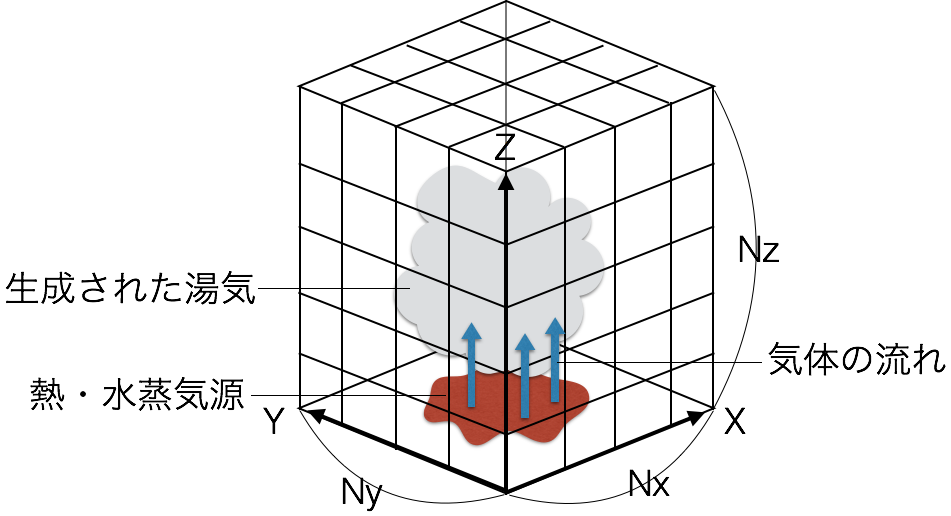
\includegraphics[width=100mm]{simulation.png}
		\caption{湯気のシミュレーション空間}
		\label{simulation}
	\end{center}
\end{figure}



